%%%%%%%%%%%%%%%%%%%%%%%%%%%%%%%%%%%%%%%%%%%%%%%%%%%%%%%%%%%%%%%%%%%%%%%%%%%%%%%%
%%%%%%%%%%%%%%%%%%%%%%%%%%%%%%%%%%%%%%%%%%%%%%%%%%%%%%%%%%%%%%%%%%%%%%%%%%%%%%%%
%%% Template for AIMS Rwanda Assignments         %%%              %%%
%%% Author:   AIMS Rwanda tutors                             %%%   ###        %%%
%%% Email: tutors2017-18@aims.ac.rw                               %%%   ###        %%%
%%% Copyright: This template was designed to be used for    %%% #######      %%%
%%% the assignments at AIMS Rwanda during the academic year %%%   ###        %%%
%%% 2017-2018.                                              %%%   #########  %%%
%%% You are free to alter any part of this document for     %%%   ###   ###  %%%
%%% yourself and for distribution.                          %%%   ###   ###  %%%
%%%                                                         %%%              %%%
%%%%%%%%%%%%%%%%%%%%%%%%%%%%%%%%%%%%%%%%%%%%%%%%%%%%%%%%%%%%%%%%%%%%%%%%%%%%%%%%
%%%%%%%%%%%%%%%%%%%%%%%%%%%%%%%%%%%%%%%%%%%%%%%%%%%%%%%%%%%%%%%%%%%%%%%%%%%%%%%%


%%%%%% Ensure that you do not write the questions before each of the solutions because it is not necessary. %%%%%% 

\documentclass[12pt,a4paper]{article}

%%%%%%%%%%%%%%%%%%%%%%%%% packages %%%%%%%%%%%%%%%%%%%%%%%%
\usepackage{amsmath}
\usepackage{amssymb}
\usepackage{amsthm}
\usepackage{amsfonts}
\usepackage{graphicx}
\usepackage[all]{xy}
\usepackage{tikz}
\usepackage{verbatim}
\usepackage{float}
\usepackage[left=2cm,right=2cm,top=3cm,bottom=2.5cm]{geometry}
\usepackage{hyperref}
\usepackage{caption}
\usepackage{subcaption}
\usepackage{psfrag}
\usepackage{mathrsfs}
\usepackage{actuarialangle}
\usepackage[T1]{fontenc}
\usepackage{setspace}
%%%%%%%%%%%%%%%%%%%%% students data %%%%%%%%%%%%%%%%%%%%%%%%
\newcommand{\student}{Yusuf Brima}
\newcommand{\course}{Mathematical Finance}
\newcommand{\assignment}{2}

%%%%%%%%%%%%%%%%%%% using theorem style %%%%%%%%%%%%%%%%%%%%
\newtheorem{thm}{Theorem}
\newtheorem{lem}[thm]{Lemma}
\newtheorem{defn}[thm]{Definition}
\newtheorem{exa}[thm]{Example}
\newtheorem{rem}[thm]{Remark}
\newtheorem{coro}[thm]{Corollary}
\newtheorem{quest}{Question}[section]

%%%%%%%%%%%%%%  Shortcut for usual set of numbers  %%%%%%%%%%%

\newcommand{\N}{\mathbb{N}}
\newcommand{\Z}{\mathbb{Z}}
\newcommand{\Q}{\mathbb{Q}}
\newcommand{\R}{\mathbb{R}}
\newcommand{\C}{\mathbb{C}}

%%%%%%%%%%%%%%%%%%%%%%%%%%%%%%%%%%%%%%%%%%%%%%%%%%%%%%%555
\begin{document}

%%%%%%%%%%%%%%%%%%%%%%% title page %%%%%%%%%%%%%%%%%%%%%%%%%%
\thispagestyle{empty}
%\begin{figure}
%    \centering
%    \includegraphics[width=\textwidth]{aims_rwanda.jpg}
%\end{figure}
\begin{center}
\textbf{AFRICAN INSTITUTE FOR MATHEMATICAL SCIENCES \\[0.5cm]
(AIMS RWANDA, KIGALI)}
\vspace{1.0cm}
\end{center}

%%%%%%%%%%%%%%%%%%%%% assignment information %%%%%%%%%%%%%%%%
\noindent
\rule{17cm}{0.2cm}\\[0.3cm]
Name: \student \hfill Assignment Number: \assignment\\[0.1cm]
Course: \course \hfill Date: \today\\
\rule{17cm}{0.05cm}
\vspace{1.0cm}
\section*{Exercise 1}
	Given a world in which there are only two risky assets $S_1$ and $S_2$, with respective expected returns.
	  \begin{spacing}{2.125}
		$
			\bar{R}_1  =  0.1  =  \frac{10}{100},	\quad \bar{R}_2  =  0.18  = \frac{18}{100}
		$
	\end{spacing}
  and variances and covariances given by
  \begin{spacing}{2.125}
  		  $
		\sigma^1_1  =  0.016  = \frac{16}{10000}, \quad \sigma_{12}^2 = 0.016  = \frac{16}{10000},\quad \sigma_2  =  0.01 =  \frac{1}{100}  
  $
  \end{spacing}
  where the opportunity set in
  \begin{spacing}{2.125}
  		 $\left(  \bar{R} ,  \sigma  \right)$ space
  \end{spacing}
The Market Price of Risk ( \textbf{MPR}) is given by 
  \begin{equation}
  		 		\theta  =  \frac{  \bar{ R}_{AC}  -  R_B }{ \sigma_{AC}}
  		 		\label{eq:mpr}
  \end{equation}
From \eqref{eq:mpr}, hte MPR is thus:
\begin{align*}
		\theta  =  \frac{\sqrt{49728}}{168}
\end{align*}
\begin{align*}
	\implies x_1  =  \frac{13}{21} ,  \quad x_2  =  \frac{8}{21}
\end{align*}
  And the Mean Return $\bar{R}_{\pi}$ is given in the equation 

  		\begin{equation}
  				\bar{R}_{\pi}  =  \lambda_1 \bar{R}_1  +   \lambda_2 \bar{R}_2  \text{ where $\lambda$ is the number of shares and $\bar{R}$ is the return} 
  				\label{eq:mr}
  		\end{equation}
  	Thus
  	\begin{align*}
  			\bar{R}_{\pi}  &=   \lambda \bar{R}_1 + (1 - \lambda) \bar{R}_2\\
  									&=  \frac{10}{100} \lambda 	+ (1 - \lambda) \frac{18}{100}\\
  									&=  \frac{18}{100}  - \frac{8\lambda}{100}\\
  									&= \frac{1}{50} (9 - 4 \lambda)
  	\end{align*}
	The correlation between two asset investments is given by equation \eqref{eq:corr}.
 	\begin{equation}
 			\rho_{12}  =  \frac{\sigma_{12}}{ \sigma_1 \sigma_2  }
 				\label{eq:corr}
 	\end{equation}
 	and the Risk of Investment is given by 
 	\begin{equation}
 			\sigma_{\pi}^2  =  \lambda_1^2 \sigma_1^2   + 2 \lambda_1 \sigma_1 \lambda_2 \sigma_2 \rho_{12}  + \lambda_2^2 \sigma_2^2
 			\label{eq:var}
 	\end{equation}
 	From \eqref{eq:var} 
 	\begin{align*}
 				\sigma_{\pi}^2  &= \lambda^2 \left(   \frac{16}{1000} \right)  + 2 \lambda ( 1 -  \lambda)  \left(   \frac{16}{1000} \right)  +  \lambda^2   \left(   \frac{1}{100} \right) \\
 										&=  \frac{1}{100} \left[   \frac{16 \lambda^2 }{100} + (2 \lambda  -  2 \lambda^2)   \left( \frac{16}{100}  \right) +   1 - 2 \lambda  + \lambda^2   \right]\\
 										&= \frac{1}{10000} \left[   16 \lambda^2  + 32 \lambda - 32 \lambda^2  + 100 - 200 \lambda + 100\lambda^2   \right]\\
 										&=   \frac{1}{10000} \left[  84 \lambda^2   -  168 \lambda + 100  \right]
 	\end{align*}
 	but 
 	\begin{align*}
 			\lambda  &= \frac{  -50 \bar{R}_{\pi}  + 9 }{ 4}
 	\end{align*}
 	\begin{align*}
 			\therefore \sigma_{\pi}^2   &=   \frac{1}{10000} \left[    84 \left(  \frac{  -50 \bar{R}_{\pi}  + 9 }{ 4} \right)  - 168 \left(  \frac{  -50 \bar{R}_{\pi}  + 9 }{ 4} \right) + 100   \right]\\
 			&= \frac{1}{ 10000} \left[   \frac{84}{ 16}   \left(  81 - 900 \bar{R}_{\pi}^2   + 25000 \bar{R}_{\pi}^2 \right)   -  \frac{  1512 + 8400 \bar{ R }_{\pi}  + 400 }{ 4}   \right]\\
 			&=  \frac{1}{ 4 \times ^4}  \left[  210000\bar{R}_{\pi}^2  -  42000 \bar{R}_{\pi} + 2356   \right] \\
 			\therefore   \sigma_{\pi}^2  &= \frac{1}{400} \left[   21,000 \bar{R}_{\pi}^2 -  42,000 \bar{R}_{\pi} + 2356  \right]^{\frac{1}{2}}
 	\end{align*}
    \begin{spacing}{2.125}
    	Given $R_0  =  0.06  =  \frac{6}{100}$ and from \eqref{eq:mpr}  
  	\end{spacing}
  	\begin{align*}
					\implies  \theta &=  \frac{ 12 -  8\lambda }{  \sqrt{  84 \lambda^2  -  168 \lambda + 100  }  } \\
					      &=  (12  -  \lambda ) ( 84 \lambda^2  -  168 \lambda + 100)^{\frac{1}{2}} 
			\end{align*}
	To minimize the risk, we differentiate $\theta $ w.r.t.  $ \lambda$.
	\begin{align*}
			\frac{d\theta}{ d \lambda }  &=  (-8) ( 84 \lambda^2  -  168 \lambda + 100)^{\frac{-1}{2}}   -  \frac{1}{2} \left[ ( 12 -  \lambda) ( 168\lambda -  168) ( 84 \lambda^2  -  168 \lambda  + 100)^{-1}  \right] = 0\\
			  &=  ( 84 \lambda^2  -  168 \lambda + 100)^{\frac{-1}{2}} \left[    -8  - (6 -  4 \lambda) ( 168 \lambda  -  168)  ( 84 \lambda^2   -  168 \lambda + 100)^{-1}    \right] = 0\\
	\end{align*}
	\begin{align*}
			 ( 84 \lambda^2  -  168 \lambda + 100)^{\frac{-1}{2}}  &=   0 \quad \text{or}\\
			 -8  - (6 -  4 \lambda) ( 168 \lambda  -  168)  ( 84 \lambda^2   -  168 \lambda + 100)^{-1}     &= 0\\
	\end{align*}
	\begin{align*}
			-172 \lambda^2  + 1344 \lambda  -  800  - 1008 \lambda + 1008 + 672 \lambda^2  -  672 \lambda  &= 0\\
			-336  \lambda  + 208  &= 0\\
			\lambda  =  \frac{208}{336}\\
			\lambda  =  \frac{13}{31}
	\end{align*}
	\begin{align*}
			\therefore  \theta  &=  \frac{ 12  -  \lambda }{  \sqrt{  84 \lambda^2   + 168 \lambda  + 100   }}\\
			    &=  \frac{  12   -  \frac{  13}{  21}}{   \sqrt{   84  \left(  \frac{13}{ 21}   \right)^2    -  168 \left(  \frac{13}{ 21}  \right)   + 100   }}\\
			     &=  \frac{    7.0476}{   \sqrt{  28.190476 }}\\
			     &=   \frac{    7.0476}{  5.3094  }\\
			     &=  1.327367
	\end{align*}
	Thus 
			\begin{align*}
						\bar{R}   &=  \theta  \sigma  + R_0\\
											&=  1.327367 \sigma + 0.06
			\end{align*}
	 \begin{figure}[!h]
									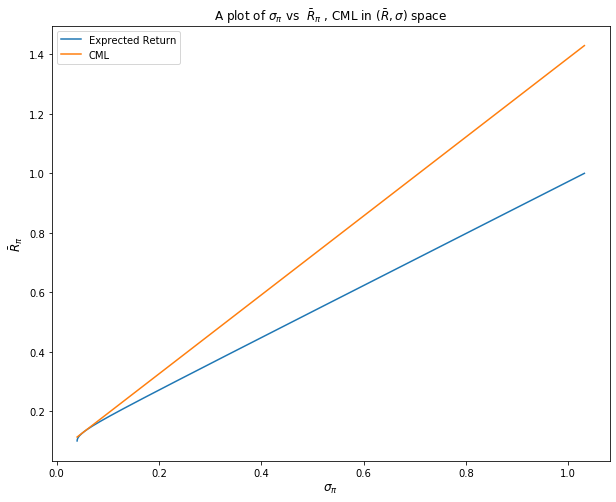
\includegraphics[width=430pt,  height=250pt]{./graphics/q001.png}
										\caption{The opportunity set in $(\bar{R}, \sigma)$ space and the efficient frontier}
										\label{fig:q1}
	\end{figure}
	\pagebreak
	\section*{Exercise 2}
			Considering a situation where there are three risky assets $S_1, S_2$ and $S_3$ with respective expected returns
			\begin{spacing}{1.125}
					$\bar{R}_1  =  0.09  =  \frac{9}{100},	\quad \bar{R}_2  =  0.11  = \frac{11}{100}, \quad \bar{R}_3  =  0.17  = \frac{17}{100}$
			\end{spacing}
			whilst the variances and covariances are given by
			\begin{spacing}{2.125}
  		  	$
				\sigma^1_1  =  0.016  = \frac{16}{10000}, \quad \sigma_{12}^2 = 				0.016  = \frac{16}{10000},  \quad \sigma_{13}^2 = 0 ,  \quad \sigma_2  =  0.01 =  \frac{1}{100} , \quad \sigma_{23}^2 =  0.012  = \frac{12}{10000},  \quad \sigma_{3}^2 = 				0.0144.  = \frac{144}{10000}, 
		  $
		  \end{spacing}
		  \begin{spacing}{2.125}
		  	If we suppose that the risk free rate $R_0  = 0.05  =  \frac{5}{100}$ and short selling and borrowing are allowed.
		  \end{spacing}
		  		  \begin{spacing}{2.125}
		  		Therefore,
		  \end{spacing}
		  \begin{align*}
		  			\sigma_{i,j}  &=  \begin{pmatrix}
		  					16 & 16 & 0 \\
		  					16 & 100 & 12\\
		  					0 & 12 & 144
		  		\end{pmatrix}\\
		  \end{align*}
		  \begin{align*}
		    &    \begin{pmatrix}
							\sigma,{1,1} & \sigma{1,2}  & \sigma{1,3}\\
							\sigma{2,1} & \sigma{2,2}  & \sigma{2,3}\\
							 \sigma{3,1} & \sigma{3,2}  & \sigma{3,3}\\
		  		\end{pmatrix} \begin{pmatrix}
		  				z_1 \\
		  				z_2\\
		  				z_3
		  		\end{pmatrix} = \begin{pmatrix}
		  				\bar{R}_1 - R_0\\
		  				\bar{R}_2 - R_0\\
		  				\bar{R}_3 - R_0
		  		\end{pmatrix}\\
		  		&   \begin{pmatrix}
		  					16 & 16 & 0 \\
		  					16 & 100 & 12\\
		  					0 & 12 & 144
		  		\end{pmatrix} \begin{pmatrix}
		  				z_1 \\
		  				z_2\\
		  				z_3
		  		\end{pmatrix} = \begin{pmatrix}
		  				\bar{R}_1 - R_0\\
		  				\bar{R}_2 - R_0\\
		  				\bar{R}_3 - R_0
		  		\end{pmatrix}\\
		  		&    \begin{pmatrix}
		  					16 & 16 & 0 \\
		  					16 & 100 & 12\\
		  					0 & 12 & 144
		  		\end{pmatrix} \begin{pmatrix}
		  				z_1 \\
		  				z_2\\
		  				z_3
		  		\end{pmatrix} = \begin{pmatrix}
							4\\ 6 \\ 12
		  		\end{pmatrix}
		  \end{align*}
			\begin{align*}
					z_1  =  \frac{79}{332}, \quad z_2  =  \frac{1}{83}, \quad z_3 =  \frac{41}{490}
			\end{align*}
			Afterwards, we find the value of $\lambda$  as follows
			\begin{spacing}{2.125}
				however,  
				 \begin{equation}
				 		z_1 + z_2 + z_3   = \lambda
				 			\label{eq:lamsum}
				 \end{equation}
				 from \eqref{eq:lamsum}
				 \begin{align*}
				 			\lambda  =  \frac{79}{332} +  \frac{1}{83} + \frac{41}{490}\\
				 				&=  \frac{331}{ 996}
				 \end{align*}
			\end{spacing}
			Then we proceed to find the values of $x_i$ s.t.  $\forall i \in \{3\}$
			\begin{align*}
					x_1  &=  \frac{z_1}{ \lambda}  = \frac{237}{ 331}\\
					x_2  &=  \frac{z_2}{ \lambda}  = \frac{12}{ 331}\\
					x_3  &=  \frac{z_3}{ \lambda}  = \frac{82}{ 331}
			\end{align*}
			It therefore follows that:
			\begin{equation*}
						x_1 + x_2 + x_3  =  1 \text{ Proved.}
			\end{equation*}
			\begin{spacing}{2.125}
						The Mean of Return $\bar{R}_{\pi}$ is thus
						\begin{align*}
								\bar{R}_{\pi}  &=  x_1 \lambda_1 + x_2  \lambda_2 + x_3 \lambda_3\\
										& =  \frac{237}{ 331} \frac{132}{ 3300} + \frac{12}{ 331} \frac{11}{100} + \frac{82}{ 331} \frac{17}{100}\\
										&=  0.1105 =  11.05 \%
						\end{align*}
			\end{spacing}
		\begin{align*}
							\sigma_{\pi}^2  & =   x_1^2  \lambda_1^2   + 2 \lambda_1 x_1  \lambda_2 x_2 \rho_{12}     + x_2^2 \lambda_2^2  + 2 x_2 \lambda_2  x_3 \lambda_3  \rho_{23} + x_3^2 \lambda_3^2 \\
							&=  0.00082  + 0.00083 + 0.000013 + 0.000022 + 0.00088\\
						\therefore \sigma_{\pi} &= 0.04268  \quad	\text{ after taking square root of both sides}
					\end{align*}
					We find the Shape Ratio as follows
					\begin{equation}
							\theta  =  \frac{  \bar{R} _{\pi}  -  R_0}{   \sigma_{\pi}}
							\label{eq:shape_ra}
					\end{equation}
				From \eqref{eq:shape_ra}
				\begin{align*}
						\implies \theta  &=  \frac{  0.1105   -  0.05}{  \sqrt{ 0.0001822}  }\\
						&=  1.1475 \approx  1.418
				\end{align*}
\section*{Exercise 3}
A pension fund manager requires an expected return of $ R\%$ with minimum risk on an investment in two risky assets $S_1$ and $S_2$ with respective expected returns
\begin{spacing}{2.125}
		$\bar{R}_1   = 0.06  =  \frac{6}{100},  \quad   \bar{R}_2   = 0.08   =  \frac{8}{100}$
\end{spacing}
with variances and covariances (scaled by $10^4$ ) given by
\begin{spacing}{2.125}
		$ \sigma_1^2  =  1 , \quad \sigma_{12}^2  =  2, \quad \sigma_2^2  =  2$
\end{spacing}
we note that 
\begin{align*}
		\lambda_1 + \lambda_2  &=  1\\
	   \implies  \lambda_1 + \lambda_2  -1  &=  10
\end{align*}
Expected return  is 
\begin{align*}
			\bar{R}_{\pi}  &=  x_1 \lambda_1 + x_2  \lambda_2\\
			  &= 6 \lambda_1  + 8 \lambda_2 \\
			 & \implies    6 \lambda_1  + 8 \lambda_2 - R =  0
\end{align*}
Risk of Investment
\begin{align*}
 			\sigma_{\pi}^2  &=  \lambda_1^2 \sigma_1^2   + 2 \lambda_1 \sigma_1 \lambda_2 \sigma_2 \rho_{12}  + \lambda_2^2 \sigma_2^2\\
 			&=  \lambda_1^2  + 4 \lambda_1 \lambda_2  \sigma_{12}  + 2 \lambda_2^2 \\
\end{align*}
\begin{align*}
		\mathcal{L} \left(  \lambda_1, \lambda_2, \alpha, \beta  \right) &=   \lambda_1^2  + 4 \lambda_1 \lambda_2  \sigma_{12}  + 2 \lambda_2^2 +  \alpha \left(  \lambda_1 + \lambda_2 -  1  \right)  + \beta \left(6 \lambda_1  + 8 \lambda_2  -  R   \right)\\
\end{align*}
We Take the partial derivatives of $\lambda_1,  \lambda_2 , \alpha,  \beta$ 
\begin{align*}
		\frac{ \partial \mathcal{L}  }{  \partial \lambda_1}   &=  2 \lambda_1  + 4 \lambda_2  + \alpha + 6 \beta  = 0\\
		&=  2 \lambda_1  + 4 \lambda_2 =  - \alpha -  6 \beta 
\end{align*}
\begin{align*}
		\frac{ \partial \mathcal{L}  }{  \partial \lambda_2}   &= 4 \lambda_1  + 4 \lambda_2 + \alpha + 8  \beta =  0\\
		 &= 4 \lambda_1  + 4 \lambda_2  = - \alpha -  8  \beta\\
\end{align*}
\begin{align*}
		\frac{ \partial \mathcal{L}  }{  \partial \alpha}   &=   \lambda_1 + \lambda_2  -  1 = 0\\
		&= \lambda_1  + \lambda_2  =  1
\end{align*}
\begin{align*}
		\frac{ \partial \mathcal{L}  }{  \partial \beta}   &=   6\lambda_1 + 8 \lambda_2  -  R  = 0\\
		&=6 \lambda_1  + 8\lambda_2  =  R
\end{align*}
Using the partial derivatives $ \frac{ \partial \mathcal{L}  }{  \partial \lambda_1} ,  \frac{ \partial \mathcal{L}  }{  \partial \lambda_2}$ we form the following system of equations.
\begin{eqnarray}
			\label{eq:simalpha}
		2 \lambda_1  + 4 \lambda_2 =  - \alpha -  6 \beta \\
		\label{eq:simbeta}
		4 \lambda_1  + 4 \lambda_2  = - \alpha -  8  \beta
\end{eqnarray}
where 
\begin{align*}
		2 \lambda_1  &=  -2 \beta \implies \lambda_1  =  -\beta\\
		\text{ and}\\
		4 \lambda_2   &=  - \alpha  - 4\beta \\
	  \lambda_2  &=  - \frac{1}{4} \alpha  -  \beta
\end{align*}
using the other system partial derivatives of $\alpha,  \beta $ we derive the following system of linear simultaneous equations.
\begin{eqnarray}
	     \lambda_1  + \lambda_2  =  1\\
     6 \lambda_1  + 8\lambda_2  =  R
\end{eqnarray}
\begin{align*}
	-6 \beta  +  8(\frac{-1}{4} \alpha  -  \beta )   &=  R\\
	-2\alpha   -  14 \beta  &= R 
\end{align*}
from \eqref{eq:simalpha},  we substitute for $ \lambda_1 $ and $ \lambda_2 $.
\begin{align*}
		-\beta  + \frac{-1}{4} \alpha  -  \beta  &= 1\\
		\frac{-1}{4} \alpha  -  2 \beta  &=  1
		-\alpha - 8\beta &=  4\\
		\therefore  -2 \alpha  -  14 \beta   =  R \quad \text{......... c}\\
		   -\alpha  - 8\beta  &=  4  \quad \text{......... d}
\end{align*} 
For (c) -  2(d)  $\implies $
\begin{align*}
		2\beta  &=  R  - 8 \\
		\therefore  \beta  &=  \frac{R}{2} - 4
\end{align*}
Also from (d)
\begin{align*}
-\alpha  - \left( 8 \frac{R}{2}  - 4   \right) &=  4\\
-\alpha  - 4R  + 32  &= 4\\
-\alpha  - 4R  &= -28\\
\alpha  &=  28 -  4R
\end{align*}
\begin{align*}
	\therefore  \lambda_1   &= -  \beta \\
	\implies \lambda_1  &=  - \left(  \frac{R}{2}    - 4  \right)\\
\end{align*}
For $ \lambda_1 \ge 0 \quad \frac{R}{2}  \le 4 \quad \implies R  \le 8 $
\begin{spacing}{1.4}
		Also 
\end{spacing}
\begin{align*}
		\lambda_2    &=  - \beta  -  \frac{\alpha}{ 4} \\
		&=  \left(   \frac{\alpha}{ 2}    \right)  -  \frac{1}{4} \left(  28 - 4R  \right)\\
		&=  4  -  \frac{R}{2}    -  \frac{28}{4} + R\\
		\lambda_2  &=  \frac{R}{2}  -3 
\end{align*}
For   $\lambda_2  \ge 0,  \quad  \frac{R}{2}  \ge 3,  \quad R \ge 6.$
\begin{spacing}{1.2}
		$\therefore  6 \le R  \le 8 $
\end{spacing}
The condition sufficiently satisfy  the constraint that prohibits short selling.
\section*{Exercise 4}
\begin{enumerate}
	\item[(a)] 
		\begin{equation}
        P(R\leq -t) = 1-c
        \label{eq:p4}
    \end{equation}
    After substituting $R$   in \eqref{eq:p4} we obtain the follow:
    \begin{align*}
        P(Q\times X\le -t) =& 1-c\\
        P(Q\{\mu + \sigma \mathcal{N}(0,1)\} \le -t)  =& 1-c\\
        P(\mu +\sigma \mathcal{N}[0,1] \le - \frac{t}{Q}) =& 1-c\\
        P ( \mathcal{N}(0,1)\leq -\frac{t}{Q\sigma} - \frac{\mu}{\sigma} ) =& 1-c\\
        \Phi\bigg( -\bigg( \frac{t}{Q \sigma} + \frac{\mu}{\sigma}\bigg)\bigg) =& 1-c\\
        1 - \Phi\bigg(\bigg( \frac{t}{Q \sigma} + \frac{\mu}{\sigma}\bigg)\bigg) =& 1-c\\
        \Phi\bigg( \bigg( \frac{t}{Q \sigma} + \frac{\mu}{\sigma}\bigg)\bigg) =& c\\
        \frac{t}{\sigma Q} + \frac{\mu}{\sigma} = & \Phi^{-1} (c)
    \end{align*}
    \begin{align*}
    		   \text{However } \quad  \Phi^{-1} (-t)  = 1- \Phi (t)\
        t + Q\mu = & Q \sigma \Phi^{-1} (c)\\
        \therefore \quad \quad t = & Q\bigg( \sigma \Phi^{-1}(c) - \mu  \bigg)\\
    \end{align*}
Thus proved.
\begin{spacing}{1.7}
	 The mean and variance for Netflix  over the period (2017, 1, 1) to (2020, 1, 1) and  the 1-day Value at Risk at the 95\% confidence level of an investment of 1,000\$.
	 \begin{verbatim}
	-----------------------------------
				Value-at-Risk: $36.878877
		-----------------------------------
				Mean is: $0.0015091
		-----------------------------------
				Variance is: $0.023338
		-----------------------------------
	 \end{verbatim}
\end{spacing}
\end{enumerate}
\end{document}